\chapter*{Introduzione}
\label{intro}
\addcontentsline{toc}{chapter}{Introduzione}

L'analisi dei segnali \`e un aspetto fondamentale per la cultura moderna: grazie
ad essa esistono telefoni, radio, televisioni, Internet e tanto altro. Grazie
all'analisi dei segnali \`e possibile riprodurre, modificare e creare audio,
immagini, video e tanto altro con l'utilizzo di un computer. Inoltre lo studio
dei segnali elettromagnetici permette di capire molto meglio il mondo attorno a
noi ed ha aperto nuove possibilit\`a per lo studio dei corpi celesti: osservare
un pianeta con il solo ausilio di strumenti ottici, infatti, non permette di
cogliere moltissimi aspetti che possiamo dedurre dallo studio degli spettri
elettromagnetici provenienti da quello stesso pianeta. Inoltre lo studio dei
buchi neri e delle stelle di neutroni non sarebbe possibile senza l'analisi dei
segnali, con cui siamo in grado di capire molto di pi\`u la loro natura e la
natura della materia in genere.

L'analisi dei segnali con mezzi informatici \`e precedente all'introduzione di
personal computers: gran parte di questo lavoro viene svolto su circuiti
elettronici costruiti su misura per effettuare le operazioni necessarie, senza
il bisogno di un calcolatore generico e di programmazione software. Questa
soluzione, ancora largamente in uso al giorno d'oggi, permette di ottenere delle
prestazioni altissime, ma ha il grande difetto di essere poco flessibile e molto
costosa: una piccola modifica quasi insignificante all'algoritmo pu\`o
significare ore e ore di lavoro specializzato. Per questo motivo si cercano al
giorno d'oggi delle soluzioni software in grado di ottenere delle prestazioni
sufficientemente buone da poter fare a meno di elaboratori DSP, cos\`i che si
possa sostituire almeno in parte questo hardware specializzato con generici
elaboratori. Il progetto sviluppato nasce proprio nell'ottica di ottenere buone
prestazioni da un normale elaboratore allo scopo di abbattere i costi in alcuni
campi di ricerca.
\section*{L'Istituto di Radioastronomia di Medicina}
\begin{figure}[htb]
	\begin{center}
		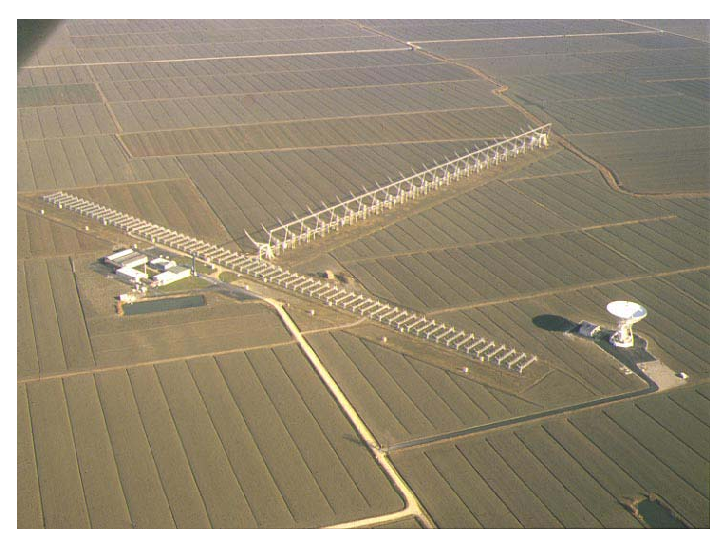
\includegraphics[width=1\linewidth]{antenne}
	\end{center}
	\caption{Veduta aerea della Croce del Nord e dell'antenna parabolica VLBI}
	\label{fig:rtscopes}
\end{figure}
Inaugurata nel 1964, la stazione ``Croce del Nord'' di Medicina (BO) ha sancito
l'inizio dell'osservazione radioastronomica in Italia, essendo il primo
osservatorio astronomico fornita di radiotelescopio invece di telescopi ottici.
Un radiotelescopio, a differenza di un telescopio ottico, non osserva i corpi
celesti tramite la parte visibile dello spettro elettromagnetico, ma li osserva
attraverso la captazione di onde radio e la loro trasformazione in segnali
elettrici. Questi segnali elettrici vengono poi elaborati per permettere
l'analisi dello spettro elettromagnetico degli oggetti osservati. I
radiotelescopi presenti a Medicina sono due: una \`e la ``Croce del Nord'', che
d\`a il nome alla stazione, formata da due serie di antenne; l'altra \`e
l'antenna parabolica \ac{VLBI}, dal diametro di 32 metri.

La ``Croce del Nord'' \`e orientata con un braccio in direzione Est-Ovest (E-W)
e l'altro braccio in direzione Nord-Sud (N-S). Il braccio E-W \`e costituito da
un'unica antenna lunga 564 metri e larga 35 metri, di forma parabolica, mentre
il braccio N-S \`e composto da 64 antenne lunghe 23,5 metri e larghe 8. La
``Croce del Nord'' lavora su segnali centrati a 408 Mhz, con larghezza di banda
che varia dai 2,5 ai 16 Mhz. La sua sensibilit\`a a segnali anche piuttosto
deboli la rende molto utile nello studio di corpi molto distanti, al di fuori
della nostra galassia. Potendo ruotare in una unica direzione, questo
radioscopio pu\`o osservare solamente segnali che transitano sulla verticale del
meridiano in cui si trova, cio\`e \`e un radiotelescopio di \emph{transito}.

L'antenna parabolica \ac{VLBI}, invece, pu\`o essere orientata in tutte le
direzioni e per questo motivo \`e possibile osservare tutti gli oggetti celesti
presenti nel cielo visibile. Questa antenna, con un diametro di 32 metri, lavora
con frequenze comprese tra i 327 Mhz ed i 43 Ghz. Ha due principali modalit\`a
operative: in rete o in \emph{single dish}.

La parabola partecipa al progetto \ac{VLBI} che, tramite la rilevazione
simultanea di diverse antenne paraboliche situate in posti diversi, permette di
raggiungere una precisione maggiore: correlando i risultati dei diversi
radiotelescopi si riesce ad ottenere una risoluzione equivalente ad una antenna
di dimensione pari alla distanza delle antenne coinvolte. Le osservazioni
particolarmente interessanti da effettuare in questa maniera sono due: la prima
prevede l'osservazione di un stesso oggetto noto da parte di radiotelescopi
situati su placche tettoniche diverse, in modo da studiare il fenomeno della
deriva dei continenti; il secondo prevede l'osservazione della posizione e delle
propriet\`a chimico-fisiche di un corpo celeste. Durante circa 4 mesi all'anno
l'antenna parabolica di Medicina \`e riservata al progetto \ac{VLBI}.

Nella modalit\`a \emph{single dish} l'antenna parabolica viene utilizzata in
modo indipendente rispetto ad altre antenne, senza correlare i dati rilevati con
altri dati. In questa modalit\`a si effettuano ad esempio ricerche di comete e
il progetto \ac{seti}.

\section*{Il progetto \ac{seti}}
Nel 1959 due fisici, Giuseppe Cocconi e Philip Morrison, pubblicarono su
\emph{Nature} un articolo in cui ponevano le basi teoriche con cui condurre
ricerche su forme di vita intelligenti extra-terrestri. Secondo questi due
scienziati, se una civilt\`a extra-terrestre evoluta volesse mettersi in
contatto con altri mondi, invierebbe segnali a banda stretta alla frequenza di
1420 Mhz: questa frequenza corrisponde all'emissione spontanea di radiazione
degli atomi di idrogeno neutro, l'elemento pi\`u diffuso nell'universo e il
pi\`u importante sotto molti aspetti di ricerca astronomica. Questa frequenza ha
anche il vantaggio di essere poco soggetta al rumore di fondo presente
nell'universo, quindi di riuscire a viaggiare a grande distanza. Inoltre un
segnale a banda stretta \`e riconosibile molto facilmente rispetto ai segnali a
banda larga emessi naturalmente dai corpi celesti, quindi la ricezione di un
segnale a banda stretta ha buone probabilit\`a di indicare una qualche emissione
artificiale.

In seguito all'articolo di Cocconi e Morrison, nel 1960 Frank Drake punt\`o un
radiotelescopio sulle stelle Tau Ceti ed Epsilon Erinadi: queste due stelle sono
di dimensioni simili al sole ed hanno probabilmente un sistema planetario simile
al sistema solare, quindi hanno una certa possibilit\`a di aver sviluppato la
vita. Bench\'e la sua ricerca non produsse esiti positivi, essa gener\`o
entusiasmo nella comunit\`a astronomica e diversi progetti simili furono avviati
da appassionati durante i tempi liberi dei propri radiotelescopi.
Nel 1961 Drake propose un'equazione per valutare quante forme di vita potrebbero
essere presenti nell'universo:
\[
N = R_* \cdot f_p \cdot n_e \cdot f_l \cdot f_i \cdot f_t \cdot L
\]
Dove:
\begin{itemize}
    \item $R_*$ \`e il numero di stelle di tipo solare che nascono nell'universo
    ogni anno.
    \item $f_p$ \`e la frazione di queste stelle che possiedono un sistema
    planerario.
    \item $n_e$ \`e il numero di pianeti per ogni sistema che si trovano ad una
    distanza adeguata per renderli abitabili.
    \item $f_l$ \`e la frazione di questi pianeti che hanno forme di vita,
    seppur primitive.
    \item $f_i$ \`e la frazione di pianeti con forme di vita intelligente.
    \item $f_t$ \`e la frazione di pianeti su cui l'avanzamento tecnologico
    permette la comunicazione con altri pianeti.
    \item $L$ indica la durata media in anni di tali civilt\`a.
\end{itemize}

Nonostante le stime di Drake indichino numerose civilt\`a presenti
nell'universo, questa equazione mostra anche i grandi problemi legati alla
ricerca \ac{seti}: molte di queste variabili sono quasi impossibili da stimare
basandosi sulla nostra conoscenza attuale dell'universo e molti altri fattori
(come ad esempio la distanza dalla Terra) non sono inclusi. Nonostante questo il
progetto prende piede e negli anni '70 anche la NASA inizia ad interessarsene,
finch\'e nel 1992 non lancia il proprio progetto \ac{seti}. In seguito la NASA
se ne disinteresser\`a ed il progetto continuer\`a solamente grazie a
finanziamenti privati ed il lavoro di volontari all'interno di osservatori
radioastronomici.

\subsection*{\ac{SERENDIP}}
Analizzare i segnali per il progetto \ac{seti} richiede un sistema informatico
in grado di effettuare i calcoli e le trasformazioni necessarie. L'Universit\`a
di Berkeley, California, ha sviluppato il sistema \ac{SERENDIP}, attualmente
alla versione IV, che permette di analizzare i segnali in modalit\`a \emph{piggy
back}, cio\`e contemporaneamente ad altre elaborazioni senza modificare il
segnale originario. In questo modo non \`e necessario dedicare del tempo di
antenna al progetto \ac{seti}, ma \`e possibile fare le osservazioni durante
altri progetti di ricerca senza interferenze: questo ha permesso di abbattere
notevolmente i costi del progetto, oltre a sfruttare tutto il tempo di utilizzo
dell'antenna. Con questo spettrometro \`e possibile analizzare segnali a 24
milioni di canali con larghezza di banda di 15 Mhz.

\section*{Il progetto}
Il progetto consiste nello sviluppo di uno spettrometro, scritto nel linguaggio
di programmazione \CC, allo scopo di ottenere le migliori prestazioni possibili
sfruttando unicamente un elaboratore generico in contrapposizione ad un
processore DSP. Questo spettrometro pu\`o trovare applicazione in diversi ambiti
di ricerca, incluso il progetto \ac{seti}, dove pu\`o essere paragonato alle
prestazioni di \ac{SERENDIP} IV.

Un requisito fondamentale di questo progetto \`e che sia sufficientemente
modulare da permettere una sua estensione e per permettere l'introduzione di
filtri e altre trasformazioni sui segnali senza dover riscrivere codice gi\`a
esistente, ma sfruttando delle interfacce predefinite.

Per raggiungere questi scopi \`e stato dedicato ampio tempo alla progettazione
del software, in modo che si potesse procedere allo sviluppo con le idee chiare
sulla struttura da adottare nel progetto.

Nei capitoli seguenti verranno illustrati alcuni concetti matematici di base
fondamentali per la comprensione del lavoro svolto, per poi procedere
all'analisi della fase di progettazione e quella di sviluppo. Verranno poi
mostrati i risultati raggiunti e tratte le relative conclusioni anche in
relazione agli obiettivi posti. Saranno poi indicati alcuni dei possibili
sviluppi futuri, ottimi punti di partenza per altri lavori di tesi o di
tirocinio per altri studenti.
